\begin{enumerate}[label=\thesubsection.\arabic*.,ref=\thesubsection.\theenumi]
\numberwithin{equation}{enumi}

\item Find the peak overshoot for the second order control system given by:

\begin{align}
    G(S) = \frac{100}{s^2 + 10s +100}
\end{align}

\solution
Peak overshoot ($M_p$) is defined as the deviation of the response at peak time from the final value of response.
\begin{align}
    \implies M_p = c(t_p) - c(\infty)
    \label{eq:eebtech11045_Mp}
\end{align}

Given,
\begin{align}
    G(S) = \frac{C(s)}{R(s)} = \frac{100}{s^2 + 10s +100}
\end{align}

To calculate the unit step response,
\begin{align}
    r(t) = 1 \implies R(s) = \frac{1}{s}    
\end{align}

\begin{align}
    \implies C(S) = \frac{1}{s}.\frac{100}{s^2 + 10s +100}
\end{align}

C(s) can be expanded as:
\begin{align}
    C(s) = \frac{1}{s} - \frac{s+5}{(s+5)^2 + 75} - \frac{1}{\sqrt{3}}.\frac{\sqrt{75}}{(s+5)^2 + 75}
\end{align}

\begin{align}
    c(t) = \mathcal{L}^{-1}{C(s)}
\end{align}

\begin{align}
    \implies c(t) = 1 - e^{-5t}\cos\brak{\sqrt{75}t} \\ - \frac{e^{-5t}}{\sqrt{3}}.\sin\brak{\sqrt{75}t}
\end{align}

c(t) can be further simplified to:
\begin{align}
    c(t) = 1 - \frac{2e^{-5t}}{\sqrt{3}}.\sin \brak{5\sqrt{3}t + \frac{\pi}{3}}
    \label{eq:eebtech11045_ct}
\end{align}

From Final Value theorem:
\begin{align}
    \lim_{s \to 0} s.C(s) = \lim_{t \to \infty} c(t) 
\end{align}

\begin{align}
    \implies c(\infty) = \lim_{s \to 0} \frac{100}{s^2 + 10s +100} = 1
\end{align}

At $t_p$, $c(t)$ is maximum:
\begin{multline}
    \implies c'(t)|_{t=t_p} = \frac{10e^{-5t}}{\sqrt{3}}.\sin {\brak{5\sqrt{3}t + \frac{\pi}{3}}}  \\ - \frac{10e^{-5t}}{\sqrt{3}}.\sqrt{3}.\cos \brak{5\sqrt{3}t + \frac{\pi}{3}} = 0
\end{multline}

\begin{align}
    \implies \sin {\brak{5\sqrt{3}t + \frac{\pi}{3}}} - \sqrt{3}.\cos \brak{5\sqrt{3}t + \frac{\pi}{3}} = 0
\end{align}
    
\begin{align}
    \implies \tan \brak{5\sqrt{3}t + \frac{\pi}{3}} = \tan \brak{\frac{\pi}{3}}    
\end{align}

\begin{align}
    \implies  5\sqrt{3}t_p = n\pi
\end{align}

The maximum overshoot occurs at $n=1$:
\begin{align}
    t_p = \frac{\pi}{\sqrt{75}} = 0.36 
\end{align}

Substitute $t_p$ in \eqref{eq:eebtech11045_ct} to get $c(t_p)$:
\begin{align}
    c(t_p) = 1 + e^\frac{-\pi}{\sqrt{3}} \implies c(t_p) = 1.163
\end{align}

Substitute $c(t_p)$ and $c(\infty)$ in \eqref{eq:eebtech11045_Mp} to get peak overshoot:
\begin{align}
    M_p = 1.16 - 1 = 0.16
\end{align}

\item Verify using a Python Plot

\solution

\begin{lstlisting}
codes/ee18btech11045.py
\end{lstlisting}

\begin{figure}[!h]
    \centering
    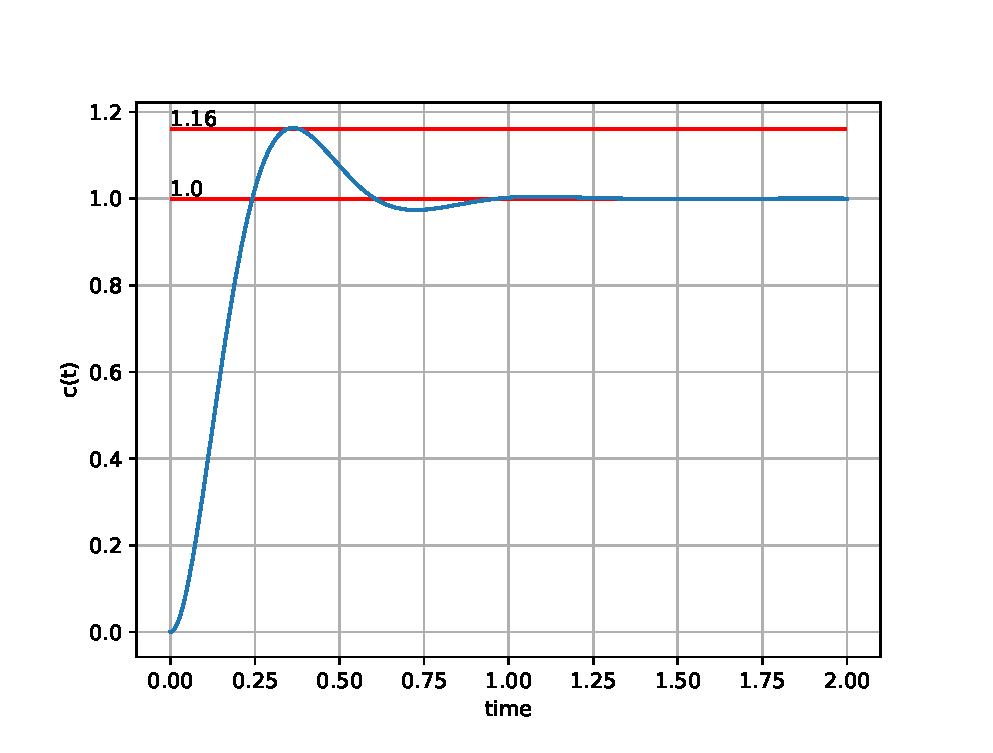
\includegraphics[width=\columnwidth]{figs/ee18btech11045/ee18btech11045.eps}
\end{figure}

\end{enumerate}